%%%%%%%%%%%%%%%%%%%%%%%%%%%%%%%%%%%%%%%%%%%%%%%%%%%%%%%%%%%%%%%%%%%%%%%%%%%%%%%%%
% Template: Article
%
% Por: Abrantes Araújo Silva Filho
%      abrantesasf@gmail.com
%
% Citação: Se você gostou deste template, por favor ajude a divulgá-lo mantendo
%          o link para meu repositório GitHub em:
%          https://github.com/abrantesasf/LaTeX
%%%%%%%%%%%%%%%%%%%%%%%%%%%%%%%%%%%%%%%%%%%%%%%%%%%%%%%%%%%%%%%%%%%%%%%%%%%%%%%%%





%%%%%%%%%%%%%%%%%%%%%%%%%%%%%%%%%%%%%%%%%%%%%%%%%%%%%%%%%%%%%%%%%%%%%%%%%%%%%%%%%
%%% Configura o tipo de documento, papel, tamanho da fonte e informações básicas
%%% para as proriedades do PDF/DVIPS e outras propriedades do documento
\RequirePackage{ifpdf}
\ifpdf
  % Classe, língua e tamanho da fonte padrão. Outras opções a considerar:
  %   draft
  %   onecolumn (padrão) ou twocolumn (OU usar o package multicol)
  %   fleqn com ou sem leqno (alinhamento à esquerda das fórmulas e dos números)
  %   oneside (padrão para article ou report) ou twoside (padrão para book)
  \documentclass[pdftex, brazil, 12pt, twoside]{article}
\else
  % Classe, língua e tamanho da fonte padrão. Outras opções a considerar:
  %   draft
  %   onecolumn (padrão) ou twocolumn (OU usar o package multicol)
  %   fleqn com ou sem leqno (alinhamento à esquerda das fórmulas e dos números)
  %   oneside (padrão para article ou report) ou twoside (padrão para book)
  \documentclass[brazil, 12pt]{article}
\fi


%%%%%%%%%%%%%%%%%%%%%%%%%%%%%%%%%%%%%%%%%%%%%%%%%%%%%%%%%%%%%%%%%%%%%%%%%%%%%%%%%
%%% Carrega pacotes iniciais necessários para estrutura de controle e para a
%%% criação e o parse de novos comandos
\usepackage{ifthen}
\usepackage{xparse}


%%%%%%%%%%%%%%%%%%%%%%%%%%%%%%%%%%%%%%%%%%%%%%%%%%%%%%%%%%%%%%%%%%%%%%%%%%%%%%%%%
%%% Configuração do tamanho da página, margens, espaçamento entrelinhas e, se
%%% necessário, ativa a indentação dos primeiros parágrafos.
\ifpdf
  \usepackage[pdftex]{geometry}
\else
  \usepackage[dvips]{geometry}
\fi
\geometry{a4paper, left=2.6cm, right=4.0cm, top=3.0cm, bottom=3.4cm}

\usepackage{setspace}
  %\singlespacing
  \onehalfspacing
  %\doublespacing


%%%%%%%%%%%%%%%%%%%%%%%%%%%%%%%%%%%%%%%%%%%%%%%%%%%%%%%%%%%%%%%%%%%%%%%%%%%%%%%%%
%%% Configurações de cabeçalho e rodapé:
\usepackage{fancyhdr}
\setlength{\headheight}{1cm}
\setlength{\footskip}{1.5cm}
\renewcommand{\headrulewidth}{0.3pt}
\renewcommand{\footrulewidth}{0.0pt}
\pagestyle{fancy}
\renewcommand{\sectionmark}[1]{%
  \markboth{\uppercase{#1}}{}}
\renewcommand{\subsectionmark}[1]{%
  \markright{\uppercase{\thesubsection \hspace{0.1cm} #1}}{}}
\fancyhead{}
\fancyfoot{}
\newcommand{\diminuifonte}{%
    \fontsize{9pt}{9}\selectfont
}
\newcommand{\aumentafonte}{%
    \fontsize{12}{12}\selectfont
}
% Configura cabeçalho e rodapé para documentos TWOSIDE
\fancyhead[EL]{\textbf{\thepage}}
\fancyhead[EC]{}
\fancyhead[ER]{\diminuifonte \textbf{\leftmark}}
\fancyhead[OR]{\textbf{\thepage}}
\fancyhead[OC]{}
\fancyhead[OL]{\diminuifonte \textbf{\rightmark}}
\fancyfoot[EL,EC,ER,OR,OC,OL]{}
% Configura cabeçalho e rodapé para documentos ONESIDE
%\lhead{ \fancyplain{}{sup esquerdo} }
%\chead{ \fancyplain{}{sup centro} }
%\rhead{ \fancyplain{}{\thesection} }
%\lfoot{ \fancyplain{}{inf esquerdo} }
%\cfoot{ \fancyplain{}{inf centro} }
%\rfoot{ \fancyplain{}{\thepage} }




%%%%%%%%%%%%%%%%%%%%%%%%%%%%%%%%%%%%%%%%%%%%%%%%%%%%%%%%%%%%%%%%%%%%%%%%%%%%%%%%%
%%% Configurações de encoding, lingua e fontes:
\usepackage[T1]{fontenc}
\usepackage[utf8]{inputenc}
\usepackage{babel}

% Altera a fonte padrão do documento (nem todas funcionam em modo math):
%   phv = Helvetica
%   ptm = Times
%   ppl = Palatino
%   pbk = bookman
%   pag = AdobeAvantGarde
%   pnc = Adobe NewCenturySchoolBook
\renewcommand{\familydefault}{ppl}


%%%%%%%%%%%%%%%%%%%%%%%%%%%%%%%%%%%%%%%%%%%%%%%%%%%%%%%%%%%%%%%%%%%%%%%%%%%%%%%%%
%%% Carrega pacotes para referências cruzadas, citações dentro do documento,
%%% links para internet e outros.Configura algumas opções.
%%% Não altere a ordem de carregamento dos packages.
\usepackage{varioref}
\ifpdf
  \usepackage[pdftex]{hyperref}
    \hypersetup{
      % Informações variáveis em cada documento (MUDE AQUI!):
      pdftitle={Internet das Coisas},
      pdfauthor={Abrantes Araújo Silva Filho},
      pdfsubject={Internet das Coisas},
      pdfkeywords={internet das coisas, internet of things, iot},
      pdfinfo={
        CreationDate={}, % Ex.: D:AAAAMMDDHH24MISS
        ModDate={}       % Ex.: D:AAAAMMDDHH24MISS
      },
      % Coisas que você não deve alterar se não souber o que está fazendo:
      unicode=true,
      pdflang={pt-BR},
      bookmarksopen=true,
      bookmarksnumbered=true,
      bookmarksopenlevel=5,
      pdfdisplaydoctitle=true,
      pdfpagemode=UseOutlines,
      pdfstartview=FitH,
      pdfcreator={LaTeX with hyperref package},
      pdfproducer={pdfTeX},
      pdfnewwindow=true,
      colorlinks=true,
      citecolor=green,
      linkcolor=red,
      filecolor=cyan,
      urlcolor=blue
    }
\else
  \usepackage{hyperref}
\fi
\usepackage{cleveref}
\usepackage{url}


%%%%%%%%%%%%%%%%%%%%%%%%%%%%%%%%%%%%%%%%%%%%%%%%%%%%%%%%%%%%%%%%%%%%%%%%%%%%%%%%%
%%% Referências bibliográficas
\usepackage[round, semicolon, authoryear]{natbib}
\bibliographystyle{abrantesasf}


%%%%%%%%%%%%%%%%%%%%%%%%%%%%%%%%%%%%%%%%%%%%%%%%%%%%%%%%%%%%%%%%%%%%%%%%%%%%%%%%%
%%% Várias notas de rodapé no mesmo local
%\usepackage[multiple]{footmisc}


%%%%%%%%%%%%%%%%%%%%%%%%%%%%%%%%%%%%%%%%%%%%%%%%%%%%%%%%%%%%%%%%%%%%%%%%%%%%%%%%%
%%% Carrega bibliotecas de símbolos (matemáticos, físicos, etc.), fontes
%%% adicionais, e configura algumas opções
\usepackage{amsmath}
\usepackage{amssymb}
\usepackage{amsfonts}
\usepackage{siunitx}
  \sisetup{group-separator = {.}}
  \sisetup{group-digits = {false}}
  \sisetup{output-decimal-marker = {,}}

% Altera separador decimal via comando, se necessário (prefira o siunitx):
%\mathchardef\period=\mathcode`.
%\DeclareMathSymbol{.}{\mathord}{letters}{"3B}
  

%%%%%%%%%%%%%%%%%%%%%%%%%%%%%%%%%%%%%%%%%%%%%%%%%%%%%%%%%%%%%%%%%%%%%%%%%%%%%%%%%
%%% Carrega packages relacionados à computação
\usepackage{algorithm2e}
\usepackage{algorithmicx}
\usepackage{algpseudocode}
\usepackage{listings}
  \lstset{literate=
    {á}{{\'a}}1 {é}{{\'e}}1 {í}{{\'i}}1 {ó}{{\'o}}1 {ú}{{\'u}}1
    {Á}{{\'A}}1 {É}{{\'E}}1 {Í}{{\'I}}1 {Ó}{{\'O}}1 {Ú}{{\'U}}1
    {à}{{\`a}}1 {è}{{\`e}}1 {ì}{{\`i}}1 {ò}{{\`o}}1 {ù}{{\`u}}1
    {À}{{\`A}}1 {È}{{\'E}}1 {Ì}{{\`I}}1 {Ò}{{\`O}}1 {Ù}{{\`U}}1
    {ä}{{\"a}}1 {ë}{{\"e}}1 {ï}{{\"i}}1 {ö}{{\"o}}1 {ü}{{\"u}}1
    {Ä}{{\"A}}1 {Ë}{{\"E}}1 {Ï}{{\"I}}1 {Ö}{{\"O}}1 {Ü}{{\"U}}1
    {â}{{\^a}}1 {ê}{{\^e}}1 {î}{{\^i}}1 {ô}{{\^o}}1 {û}{{\^u}}1
    {Â}{{\^A}}1 {Ê}{{\^E}}1 {Î}{{\^I}}1 {Ô}{{\^O}}1 {Û}{{\^U}}1
    {œ}{{\oe}}1 {Œ}{{\OE}}1 {æ}{{\ae}}1 {Æ}{{\AE}}1 {ß}{{\ss}}1
    {ű}{{\H{u}}}1 {Ű}{{\H{U}}}1 {ő}{{\H{o}}}1 {Ő}{{\H{O}}}1
    {ç}{{\c c}}1 {Ç}{{\c C}}1 {ø}{{\o}}1 {å}{{\r a}}1 {Å}{{\r A}}1
    {€}{{\euro}}1 {£}{{\pounds}}1 {«}{{\guillemotleft}}1
    {»}{{\guillemotright}}1 {ñ}{{\~n}}1 {Ñ}{{\~N}}1 {¿}{{?`}}1
  }
  

%%%%%%%%%%%%%%%%%%%%%%%%%%%%%%%%%%%%%%%%%%%%%%%%%%%%%%%%%%%%%%%%%%%%%%%%%%%%%%%%%
%%% Ativa suporte extendido a cores
\usepackage[svgnames]{xcolor} % Opções de cores: usenames (16), dvipsnames (64),
                              % svgnames (150) e x11names (300).


%%%%%%%%%%%%%%%%%%%%%%%%%%%%%%%%%%%%%%%%%%%%%%%%%%%%%%%%%%%%%%%%%%%%%%%%%%%%%%%%%
%%% Suporte à importação de gráficos externos
\ifpdf
  \usepackage[pdftex]{graphicx}
\else
  \usepackage[dvips]{graphicx}
\fi


%%%%%%%%%%%%%%%%%%%%%%%%%%%%%%%%%%%%%%%%%%%%%%%%%%%%%%%%%%%%%%%%%%%%%%%%%%%%%%%%%
%%% Suporte à criação de gráficos proceduralmente na LaTeX:
\usepackage{tikz}
  \usetikzlibrary{arrows,automata,backgrounds,matrix,patterns,positioning,shapes,shadows}


%%%%%%%%%%%%%%%%%%%%%%%%%%%%%%%%%%%%%%%%%%%%%%%%%%%%%%%%%%%%%%%%%%%%%%%%%%%%%%%%%
%%% Packages para tabelas
\usepackage{array}
\usepackage{longtable}
\usepackage{tabularx}
\usepackage{tabu}
\usepackage{lscape}
\usepackage{colortbl}  
\usepackage{booktabs}


%%%%%%%%%%%%%%%%%%%%%%%%%%%%%%%%%%%%%%%%%%%%%%%%%%%%%%%%%%%%%%%%%%%%%%%%%%%%%%%%%
%%% Packages ambientes de listas
\usepackage{enumitem}
\usepackage[ampersand]{easylist}


%%%%%%%%%%%%%%%%%%%%%%%%%%%%%%%%%%%%%%%%%%%%%%%%%%%%%%%%%%%%%%%%%%%%%%%%%%%%%%%%%
%%% Packages para suporte a ambientes floats, captions, etc.:
\usepackage{float}
\usepackage{wrapfig}
\usepackage{placeins}
\usepackage{caption}
\usepackage{sidecap}
\usepackage{subcaption}


%%%%%%%%%%%%%%%%%%%%%%%%%%%%%%%%%%%%%%%%%%%%%%%%%%%%%%%%%%%%%%%%%%%%%%%%%%%%%%%%%
%%% Meus comandos específicos:
% Commando para ``italizar´´ palavras em inglês (e outras línguas!):
\newcommand{\ingles}[1]{\textit{#1}}

% Commando para colocar o espaço correto entre um número e sua unidade:
\newcommand{\unidade}[2]{\ensuremath{#1\,\mathrm{#2}}}
\newcommand{\unidado}[2]{{#1}\,{#2}}

% Produz ordinal masculino ou feminino dependendo do segundo argumento:
\newcommand{\ordinal}[2]{%
#1%
\ifthenelse{\equal{a}{#2}}%
{\textordfeminine}%
{\textordmasculine}}


%%%%%%%%%%%%%%%%%%%%%%%%%%%%%%%%%%%%%%%%%%%%%%%%%%%%%%%%%%%%%%%%%%%%%%%%%%%%%%%%%
%%% Hifenização específica quando o LaTeX/Babel não conseguirem hifenizar:
\babelhyphenation{Git-Hub au-to-con-fi-gu-rá-vel}


%%%%%%%%%%%%%%%%%%%%%%%%%%%%%%%%%%%%%%%%%%%%%%%%%%%%%%%%%%%%%%%%%%%%%%%%%%%%%%%%%
%%%%%%%%%%%%%%%%%%%%%%%%%%%%%%%%%%%%%%%%%%%%%%%%%%%%%%%%%%%%%%%%%%%%%%%%%%%%%%%%%
%%%%%%%%%%%%%%%%%%%%%%%%%%%%%%%%%%%%%%%%%%%%%%%%%%%%%%%%%%%%%%%%%%%%%%%%%%%%%%%%%
%%%%%%%%%%%%%%%%%%%%%%%%%%%%%%%%%%%%%%%%%%%%%%%%%%%%%%%%%%%%%%%%%%%%%%%%%%%%%%%%%
%%%%%%%%%%%%%%%%%%%%%%%%%%%%%% COMEÇA O DOCUMENTO %%%%%%%%%%%%%%%%%%%%%%%%%%%%%%%
%%%%%%%%%%%%%%%%%%%%%%%%%%%%%%%%%%%%%%%%%%%%%%%%%%%%%%%%%%%%%%%%%%%%%%%%%%%%%%%%%
%%%%%%%%%%%%%%%%%%%%%%%%%%%%%%%%%%%%%%%%%%%%%%%%%%%%%%%%%%%%%%%%%%%%%%%%%%%%%%%%%
%%%%%%%%%%%%%%%%%%%%%%%%%%%%%%%%%%%%%%%%%%%%%%%%%%%%%%%%%%%%%%%%%%%%%%%%%%%%%%%%%
%%%%%%%%%%%%%%%%%%%%%%%%%%%%%%%%%%%%%%%%%%%%%%%%%%%%%%%%%%%%%%%%%%%%%%%%%%%%%%%%%
\begin{document}
\title{Internet das Coisas}
\author{Abrantes Araújo Silva Filho \and Brendhom Félix Garcia Brito
  \and Carlos Augusto Caus Couto \and Eliziel de Paula da Silva \and Iuri Alves Contarelli
  \and Victor Luchsinger Lube}
\date{2018-04-19}
\maketitle
\tableofcontents


%%%%%%%%%%%%%%%%%%%%%%%%%%%%%%%%%%%%%%%%%%%%%%%%%%%%%%%%%%%%%%%%%%%%%%%%%%%%%%%%%
%%%%%%%%%%%%%%%%%%%%%%%%%%%%%%%%%%%%%%%%%%%%%%%%%%%%%%%%%%%%%%%%%%%%%%%%%%%%%%%%%
%%%%%%%%%%%%%%%%%%%%%%%%%%%%%%%%%%%%%%%%%%%%%%%%%%%%%%%%%%%%%%%%%%%%%%%%%%%%%%%%%
\section{Introdução}
\label{intro}

Nos últimos anos a tecnologia permitiu a criação e o desenvolvimento de dispositivos com a
capacidade de se conectar à Internet e de trocar informações. Esses dispositivos,
segundo \citet{BarbozaTCCIoT2015}, ``são objetos físicos, 'coisas', que passam
a alojar sistemas eletrônicos embarcados com componentes de \ingles{software},
sensores e, principalmente conectividade, que permite a esses objetos trocarem
informações através da rede''.

Apesar de não haver um consenso na definição do campo de ``dispositivos conectados'',
o nome Internet das Coisas --- do inglês \ingles{Internet of Things} (IoT)\footnote{Neste trabalho
  usaremos o termo ``IoT'' para indicar todo o ecossistema de dispositivos conectados.} --- passou
a significar todo o ecossistema de \ingles{hardware} e \ingles{software} que
permite a conexão dos dispositivos entre si e à Internet.

A produção em escala desses dispositivos para IoT com a conseqüente queda no custo
de produção, aliado à enorme distribuição de redes de conectividade \ingles{wireless},
expandiu de forma exponencial as possibilidades de uso e lucratividade com
tal tecnologia. No ano de 2013 a Cisco estimou que esse potencial
de mercado era de 14,4 trilhões de dólares em dez anos\footnote{De 2013 a 2022, considerando
o mercado global.}~\citep{CiscoIoTFAQ2013},
e que até 2020 haverá 50,1 bilhões de dispositivos conectados à Internet,
realizando diversas tarefas e serviços~\citep{CiscoIoEConnectionsCounter}.

Além das empresas de tecnologia, grandes consultoras de negócios internacionais
já apontam o enorme potencial da IoT, explicitamente aconselhando
seus clientes a investirem na área.
A Morgan Stanley publicou dois relatórios~\citep{MorganStanleyIoTnow2013,MorganStanleyIoTpersonal2014}
que apontam enorme potencial de ganhos, e a \citet{OliverWymanIoT2015} classifica
a IoT como ``uma nova revolução capaz de romper os modelos de negócios tradicionais''.

Até mesmo governos, que geralmente são mais lentos na adoção de novas tecnologias, já
se movimentam para estudar, testar e implantar soluções concetadas. O Reino Unido,
por exemplo, estabeleceu para si a meta de se tornar, através do investimento em IoT,
a ``nação mais digital entre os componentes do G8\footnote{França, Alemanha, Reino Unido,
  Japão, Canadá, Itália, Estados Unidos e Rússia (esta foi afastada recentemente sob
  a acusação de violaão da soberania nacional da Ucrânia).}'' e 
``o líder mundial no desenvolvimento e implementação da IoT''~\citep{UKGOSWalportIoT2014}.

E por que toda essa agitação em torno da IoT? Porque as suas aplicações
são praticamente inesgotáveis, variando desde uma simples
\ingles{Smart-TV} capaz de se conectar à Internet e atualizar a programação de
filmes disponíveis ou de um simples sistema de irrigação de jardim capaz de
obter a previsão de chuva a partir de serviços na Internet e ajustar a periodicidade
na qual a grama será molhada, até dispositivos complexos como um marca-passo cardíaco
capaz de informar automaticamente ao médico ou uma equipe de emergência uma possível
disfunção miocárdica que exija tratamento imediato.

Este trabalho pretende apresentar uma visão geral do campo da IoT, incluindo os
seguintes tópicos:

\begin{itemize}[noitemsep]
\item Definições e conceitos
\item Histórico
\item Vantagens e desvantagens
\item Riscos e perigos
\item Exemplos de aplicações (que deram certo e errado)
\item Tecnologias utilizadas
\end{itemize}

Além disso este trabalho apresentará uma breve descrição de um protótipo de
cofre conectado à Internet por um Arduino\footnote{\url{https://www.arduino.cc/}},
que será desenvolvido pelos autores como uma prova de conceito da IoT.


%%%%%%%%%%%%%%%%%%%%%%%%%%%%%%%%%%%%%%%%%%%%%%%%%%%%%%%%%%%%%%%%%%%%%%%%%%%%%%%%%
%%%%%%%%%%%%%%%%%%%%%%%%%%%%%%%%%%%%%%%%%%%%%%%%%%%%%%%%%%%%%%%%%%%%%%%%%%%%%%%%%
\section{O que é IoT?}
\label{o-que-e-iot}


%%%%%%%%%%%%%%%%%%%%%%%%%%%%%%%%%%%%%%%%%%%%%%%%%%%%%%%%%%%%%%%%%%%%%%%%%%%%%%%%%
\subsection{Definição e conceitos}
\label{o-que-e-iot-definicao}

Não existe um consenso estabelecido sobre o que realmente é a IoT e qual a melhor
maneira de definí-la. Isso ocorre devido a relativa pouca idade e maturação do
campo, devido às diverentes visões dos dispositivos pioneiros de IoT, e devido
ao praticamente ilimitado potencial de uso para diferentes atividades e serviços
em diversas áreas (indústria, doméstica, saúde, financeira, engenharia e muitas
outras). Se a IoT estará presente em ``tudo'' e servirá para ``tudo'', como
definí-la precisamente?

Inicialmente vamos eliminar uma visão simplória e quase caricata da IoT: a
``geladeira conectada que compra leite fresco'' (Figura~\ref{fig:smart-geladeira}).
\citet{UKGOSWalportIoT2014}
argumenta que esse tipo de estereótipo somente contribui para ``trivializar
a importância da IoT'' e mascarar o verdadeiro potencial de impacto na sociedade.
Eletrodomésticos conectados são uma pequena parte da IoT, mas não a mais
importante.

\begin{figure}[H]
  \begin{center}
    \caption{``A porta-voz da Samsung, Kai Madden, exibe o recurso de conectividade em
      uma geladeira inteligente Samsung''~\citep{BajarinIoE2014}.}
    \label{fig:smart-geladeira}
    \fbox{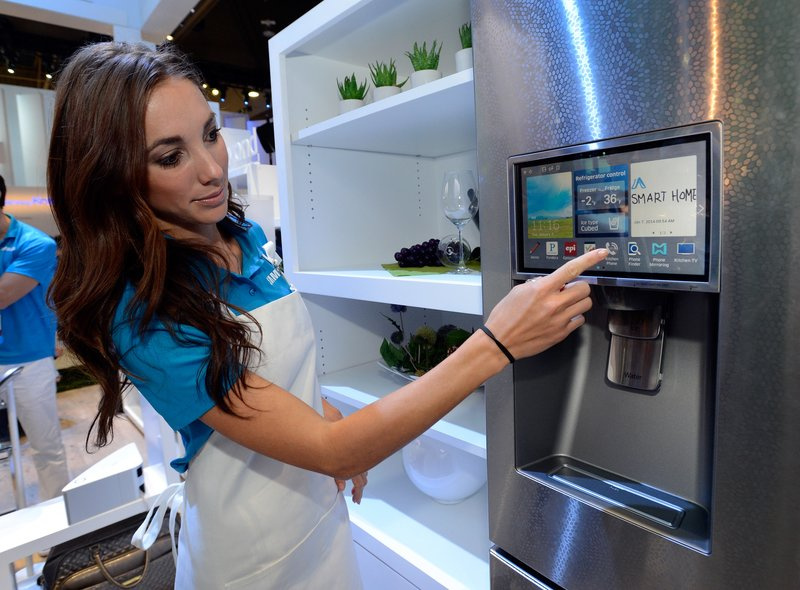
\includegraphics[scale=0.8]{imagens/geladeira.jpeg}}

    \footnotesize{Foto de David Becker, retirada do artigo de ~\citet{BajarinIoE2014},
      disponível em \url{http://time.com/539/the-next-big-thing-for-tech-the-internet-of-everything/}}
  \end{center}
\end{figure}

Se a IoT não se resume a eletrodomésticos conectados, o que ela é de fato? As
grandes empresas de tecnologia definem IoT do seguinte modo:

\begin{itemize}
\item \emph{\textbf{SAP}}: ``A Internet das Coisas é uma rede de objetos físicos --- veículos,
  máquinas, eletrodomésticos e outros --- que usam sensores e APIs para conectar e
  trocar dados na Internet''~\citep{SAPWhatIoT}.
\item \emph{\textbf{SAS}}: ``A Internet das Coisas é o conceito de objetos do cotidiano --- de
  máquinas industriais à dispositivos vestíveis ---- usando sensores embutidos para coletar
  dados e tomar uma ação sobre esses dados através da rede''\citep{SASWhatIoT}.
\item \emph{\textbf{IBM}}: ``A Internet das Coisas refere-se à variedade crescente
  de dispositivos conectados que enviam dados através da Internet. Uma 'coisa' é qualquer
  objeto com eletrônica embarcada que pode transferir dados em uma rede --- sem nenhuma
  interação humana''~\citep{IBMWhatIsIoT,IBMWhatsonIoT}.
\item \emph{\textbf{Cisco}}: ``A Internet das Coisas (IoT) refere-se simplesmente à conexão
  em rede de objetos físicos''~\citep{CiscoIoTVS2013}.
\item \emph{\textbf{Amazon}}: ``Um sistema de dispositivos ubíquos conectando o mundo
  físico à nuvem''~\citep{AmazonIoT}.
\item \emph{\textbf{Microsoft}}: embora a Microsoft não defina explicitamente o que
  ela entende por IoT, em um vídeo institucional sobre a plataforma \emph{Microsoft IoT}
  podemos deduzir que o conceito de IoT envolve conectar as partes mais vitais de
  seu negócio (pessoas, ativos, processos e sistemas), do chão de fábrica aos ``campos''
  para aumentar o alcançe da empresa e fazer melhor uso dos recursos~\citep{MicrosoftIoT}.
\item \emph{\textbf{Google}}: a empresa também não fornece uma definição explícita mas
  sua plataforma \emph{Google Cloud IoT Core} está voltada à ``conexão segura, coleta e
  gerenciamento de dados a partir de milhões de dispositivos globalmente dispersos [\ldots]
  para processar, analisar e visualizar dados em tempo real para suportar o aumento
  da eficiência operacional''~\citep{GoogleWhatsIoT}.
\end{itemize}

Um grande esforço de entendimento e conceituação da IoT foi realizado pelo \ingles{Institute
  of Electrical and Electronics Engineers (IEEE)} que, reconheceu a grande importância
do tema~\citep{IEEEIoTReport}, revisou a definição de IoT
de várias organizações, projetos de pesquisa, governos e instituições de ensino, e publicou
em 2015 sua própria definição de IoT no
relatório\footnote{\url{https://iot.ieee.org/definition.html}}\textsuperscript{, }\footnote{O IEEE revisou
  as definições e conceituações de IoT de 8 organismos internacionais de padronização, 8 projetos
  de pesquisa em IoT, 3 iniciativas de governos, 7 relatórios institucionais de empresas e
  consultorias, 5 livros que tratam exclusivamente de IoT e 3 definições fornecidas por indústrias
que lidam com IoT.}
``\ingles{Towards a definition of
  the Internet of Things (IoT)}''~\citep{IEEEIoTDefinition}. A definição proposta
pelo IEEE é a seguinte:

\begin{quote}
  ``A Internet das Coisas (IoT) é uma rede complexa, auto-configurá-vel e adaptativa,
  que interconecta 'coisas' à Internet através do uso de protocolos de comunicação
  padronizados. As coisas interconectadas têm representação física ou virtual no mundo
  digital, com capacidades sensoriais, de atuação e programabilidade, e são unicamente
  identificáveis. A representação contém informação sobre a coisa incluindo sua identidade,
  status, localização ou qualquer outra informação relevante, privada, social ou
  empresarial. A coisa oferece serviços, com ou sem a intervenção humana, através
  da exploração de sua identificação única, dados capturados, comunicação e capacidade
  de atuação. Os serviços são explorados através do uso de interfaces inteligentes e
  estão disponíveis em qualquer lugar, a qualquer hora e para qualquer um ou qualquer
  coisa, levando em consideração questões de segurança.''~\citep{IEEEIoTDefinition}
\end{quote}

Dissecando a definição da IEEE podemos compreender melhor cada parte da IoT:

\begin{enumerate}
\item \emph{\textbf{Coisa}}: é qualquer dispositivo que possa ser conectado
  à Internet, variando desde um minúsculo sensor até um carro ou outro
  grande equipamento, e que tenha capacidade sensorial, de atuação ou de
  programabilidade.
\item \emph{\textbf{Identificação única}}: cada coisa deve ser unicamente
  identificável na Internet pois só assim pode-se captar dados relevantes
  e oferecer serviços importantes para cada um.
\item \emph{\textbf{Ubiquidade}}: as coisas e os serviços por elas disponibilizados
  devem estar disponíveis em qualquer lugar, a qualquer hora e para qualquer um
  ou qualquer coisa (note-se que uma coisa pode oferecer serviços para outras
  coisas).
\item \emph{\textbf{Rede}}: as coisas conversam, trocam dados e oferecem
  serviços através de uma rede complexa, atualmente a Internet.
\item \emph{\textbf{Autonomia}}: as coisas devem ser capazes de
  obter dados e oferecer serviços sem a intervenção humana (não excluindo
  a possibilidade da participação humana ativa também).
\item \emph{\textbf{Segurança}}: toda essa atividade de coleta e troca de
  dados via rede resulta em desafios imensos relacionados à segurança e
  privacidade das informações, e as questões de segurança devem ser
  tratadas pelas coisas e seus protocolos de comunicação.
\end{enumerate}


%%%%%%%%%%%%%%%%%%%%%%%%%%%%%%%%%%%%%%%%%%%%%%%%%%%%%%%%%%%%%%%%%%%%%%%%%%%%%%%%%
\subsection{Ecossistema da IoT}
\label{o-que-e-iot-ecossistema}

Todas as ``coisas'' conectadas à internet, incluindo todo o \ingles{hardware}
e \ingles{software} formam o ``ecossistema da IoT'' (ver Figuras~\ref{fig:ecossistema1}
e \ref{fig:ecossistema2}).

O \ingles{hardware} inclui os próprios dispositivos, sensores, atuadores,
servidores de processamento, servidores de armazenamento de dados,
infra-estrutura de rede, infra-estrutura de nuvem, equipamentos de backup, etc. Enfim,
inclui tudo o que é necessário para manter a estrutura da IoT funcionando.

O \ingles{software} inlcui os sistemas embarcados nos dispositivos, os sistemas
nos servidores, os sistemas de coleta e análise de dados ou qualquer outro
sistema ou programa para que a IoT funcione adequadamente.

\begin{figure}[H]
  \begin{center}
    \caption{Ecossistema, características e escopo da IoT.}
    \label{fig:ecossistema1}
    \fbox{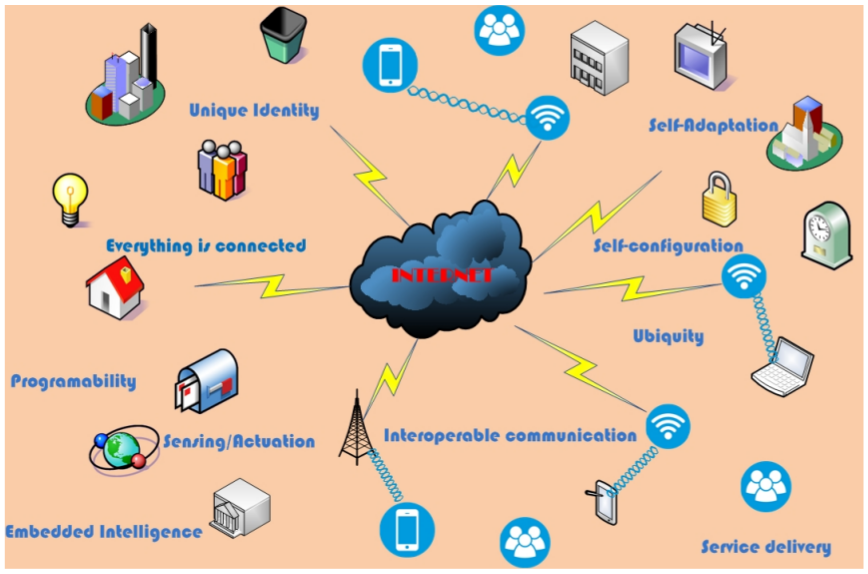
\includegraphics[scale=0.4]{imagens/ecossistema1.png}}
    
    \footnotesize{Ilustração retirada do relatório do~\citet{IEEEIoTDefinition}}
  \end{center}
\end{figure}

\begin{figure}[H]
  \begin{center}
    \caption{Ecossistema da IoT.}
    \label{fig:ecossistema2}
    \fbox{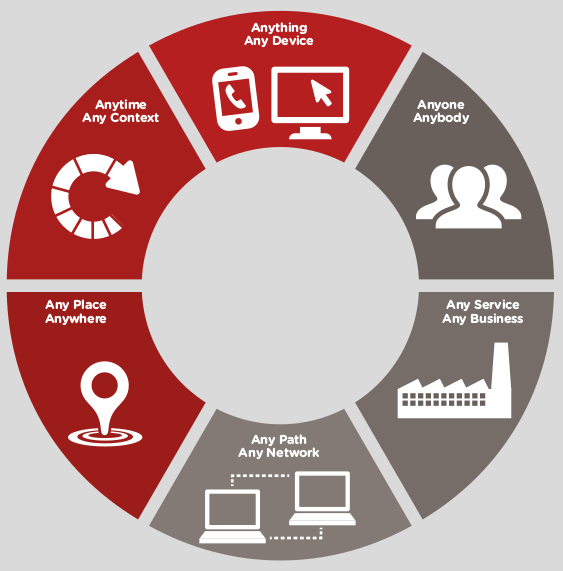
\includegraphics[scale=0.5]{imagens/ecossistema2.png}}
    
    \footnotesize{Ilustração retirada do relatório de~\citet{UKGOSWalportIoT2014}}
  \end{center}
\end{figure}

Alguns autores~\citep{UKGOSWalportIoT2014,IEEEIoTDefinition,BarbozaTCCIoT2015}
identificam, a grosso modo, dois ``tamanhos'' de ecossistema para as aplicações da IoT:
pequena ou grande escala. O que diferencia entre essas duas é a comlexidade em termos
de:

\begin{itemize}[noitemsep]
\item Número de dispositivos
\item Propriedade e gerenciamento das coisas
\end{itemize}

Um ecossistema IoT de pequena escala corresponde à uma rede de dispositivos
pouco complexa, com relativamente poucos dispositivos e, principalmente, com
um único proprietário gerenciador. Aqui se encaixam as soluções
de IoT de um único fabricante. Por exemplo: sistemas para a irrigação de jardins
que utilizam dados de previsão do tempo, sistemas em veículos que indicam ao
motorista a necessidade de manutenção preventiva, sistemas em marca-passos cardíacos
que avisam à equipe médica se algum problema ocorrer.

Por outro lado, um ecossistema IoT de grande escala corresponde à uma rede
de dispositivos muito complexa, com muitos dispositivos e, principalmente, com
diversos proprietários e gerenciadores (que podem até não ter relacionamentos
explícitos entre eles). Segundo o \citet{IEEEIoTDefinition}, ``nesse contexto,
a complexidade torna-se dominante e elementos como escalabilidade, lógica distribuída,
etc., tornam-se essenciais. Todas as abordagens tradicionais para gerenciamento
de confiança, nomeação, descoberta, etc., devem ser completamente repensadas''.

As soluções de pequena escala, apesar do nome, já causam profundo impacto na sociedade
mas o maior potencial para a IoT será quando for possível conectar todos os dispositivos,
de todos os fabricantes, em um ecossistema de grande escala~\citep{UKGOSWalportIoT2014,IEEEIoTDefinition,BhattIoT,IEEEIoTReport,McKinseyIoTHype,MoolayilIoT2016,RajIoT2017,OliverWymanIoT2015,SAPFutureIoT,CiscoIoEPublicSectorOpportunity,CiscoIoTFAQ2013,CiscoIoTVS2013,CiscoIoEPublicSectorEconomicAnalysis,CiscoIoESurvey2013,CiscoIoEValuePrivate2013,CiscoIoEValuePublic2013}.

Obviamente, apesar do grande potencial em conectar todos os dispositivos, de todos
os fabricantes, em uma grande rede comum de troca de informações e prestação de
serviços, existem grandes obstáculos a serem superados até que essa visão de futuro
possa ser alcançada \citep{UKGOSWalportIoT2014}.


%%%%%%%%%%%%%%%%%%%%%%%%%%%%%%%%%%%%%%%%%%%%%%%%%%%%%%%%%%%%%%%%%%%%%%%%%%%%%%%%%
\subsection{Breve histórico}
\label{o-que-e-iot-historia}

xxx



%%%%%%%%%%%%%%%%%%%%%%%%%%%%%%%%%%%%%%%%%%%%%%%%%%%%%%%%%%%%%%%%%%%%%%%%%%%%%%%%%
%%%%%%%%%%%%%%%%%%%%%%%%%%%%%%%%%%%%%%%%%%%%%%%%%%%%%%%%%%%%%%%%%%%%%%%%%%%%%%%%%
%%%%%%%%%%%%%%%%%%%%%%%%%%%%%%%%%%%%%%%%%%%%%%%%%%%%%%%%%%%%%%%%%%%%%%%%%%%%%%%%%
%%%%%%%%%%%%%%%%%%%%%%%%%%%%%%%%%%%%%%%%%%%%%%%%%%%%%%%%%%%%%%%%%%%%%%%%%%%%%%%%%
%%%%%%%%%%%%%%%%%%%%%%%%%%%%%% TERMINA O DOCUMENTO %%%%%%%%%%%%%%%%%%%%%%%%%%%%%%
%%%%%%%%%%%%%%%%%%%%%%%%%%%%%%%%%%%%%%%%%%%%%%%%%%%%%%%%%%%%%%%%%%%%%%%%%%%%%%%%%
%%%%%%%%%%%%%%%%%%%%%%%%%%%%%%%%%%%%%%%%%%%%%%%%%%%%%%%%%%%%%%%%%%%%%%%%%%%%%%%%%
%%%%%%%%%%%%%%%%%%%%%%%%%%%%%%%%%%%%%%%%%%%%%%%%%%%%%%%%%%%%%%%%%%%%%%%%%%%%%%%%%
%%%%%%%%%%%%%%%%%%%%%%%%%%%%%%%%%%%%%%%%%%%%%%%%%%%%%%%%%%%%%%%%%%%%%%%%%%%%%%%%%
\bibliography{/home/abrantesasf/repositoriosGit/BibTeX/biblioteca}
\end{document}
